\section{Summary of Papers}
\label{sec:summary}

\subsection{AutoNER}
AutoNER \cite{autoner} has two contributions: Fuzzy LSTM CRF and Tie-or-Break scheme.


\noindent\textbf{Fuzzy LSTM CRF}
Have to read about CRF and why they work.

\noindent\textbf{Tie-or-Break Scheme}
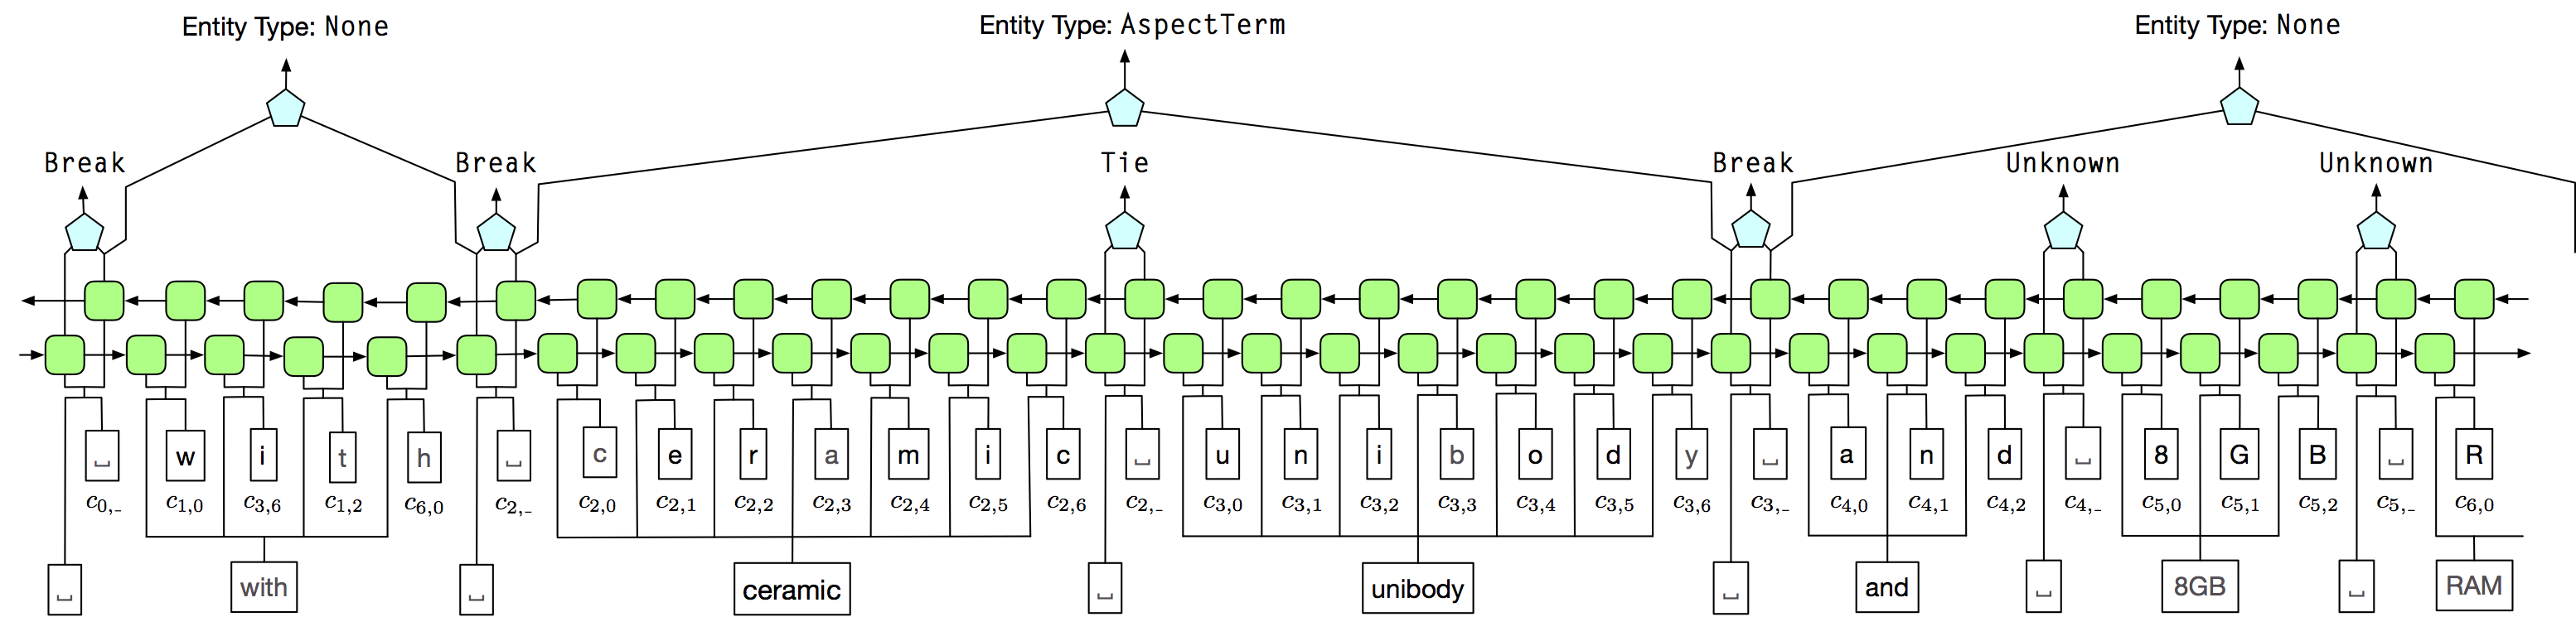
\includegraphics[scale=0.5]{images/autoner_tie_or_break.png}
